\documentclass[a4paper,10pt,french]{report}
\usepackage[french]{babel}
\usepackage[pdftex=true, colorlinks=true, linkcolor=DarkSlateBlue]{hyperref}
\usepackage[utf8]{inputenc}
\usepackage[T1]{fontenc}
\usepackage{epstopdf}
\usepackage{graphicx,graphics}
\usepackage{amsmath,amsfonts,amssymb}
\usepackage[svgnames]{xcolor}
\usepackage[top=4cm, bottom=4cm, left=2.5cm, right=2.5cm]{geometry}

\makeatletter
\renewcommand{\thesection}{\@arabic\c@section}
\makeatother

\begin{document}
\author{Antoine Wacheux et Paul Marillonnet}
\title{LO21 : Rapport de projet}\maketitle

\tableofcontents
\newpage



\section*{Indroduction}\label{sec:Introduction}\addcontentsline{toc}{section}{Introduction}

Ce rapport s'inscrit dans le cadre du projet de l'unité de valeur LO21.\\
La première partie de ce rapport concerne une description de l'architecture de l'application UTProfiler, développée à l'aide de l'IDE QtCreator, et la seconde partie se concentre davantage sur une explication, une justification des choix concernant l'architecture adoptée, notamment en ce qui concerne sa capacité à évoluer (c'est-à-dire mettant en oeuvre les notions de modularité, d'extensibilité et de réutilisabilité).

\newpage
\section{Description de l'architecture}\label{sec:I}



	\subsection{UTManager}\label{subsec:UTManager}
	
	La classe \emph{UTManager} repose sur le design pattern Singleton (d'où l'utilisation de l'abréviation \emph{sUTManager} à la place de \emph{UTManager::getInstance()}).
    Par ailleurs, comme son nom l'indique, son rôle est central dans l'application, cette classe n'est pas seulement responsable de la gestion des UV. \\
	Ce singleton met à disposition de l'utilisateur fonctionnalités nécessaires à la gestion :
	\begin{itemize}
	\item Des UV
	\item Des branches
	\item Des profils
	\item Du chargement des fichiers de données XML	
	\end{itemize}
	Ainsi, se placer à un niveau de gestion au dessus de ce qu'un manager d'UV pourrait offrir en terme de fonctionnalités permet de ne pas avoir multiplier les classes de manager d'entités (\emph{UVManager}, \emph{BrancheManager}, \emph{ProfilManager} ...)

				
	\subsection{UTStream}\label{subsec:UTStream}
	
		Il s'agit de la classe abstraite qui présente l'interface de chargement et de sauvegarde des données.
		En pratique, la classe concrête réalisant ces deux tâches est \emph{UVStreamXML}. Le modèle de données XML associé est le suivant :
		\begin{quote}

<SectionUV>\\
	\hspace*{1cm}<uv>\\
	\hspace*{1cm}	\hspace*{1cm}<code></code>\\
	\hspace*{1cm}	\hspace*{1cm}<nom></nom>\\
	\hspace*{1cm}\hspace*{1cm}	<credit type=""></credit>\\
	\hspace*{1cm}\hspace*{1cm}	<branche></branche>\\
	\hspace*{1cm}</uv>\\
</SectionUV>\\
<SectionBranche>\\
	\hspace*{1cm}<branche>\\
	\hspace*{1cm}\hspace*{1cm}	<sigle></sigle>\\
	\hspace*{1cm}\hspace*{1cm}	<nom></nom>\\
	\hspace*{1cm}\hspace*{1cm}	<PCB></PCB>\\
	\hspace*{1cm}\hspace*{1cm}	<PSF></PSF>\\
	\hspace*{1cm}</branche>\\
</SectionBranche>\\
<SectionProfil>\\
	\hspace*{1cm}<profil>\\
	\hspace*{1cm}\hspace*{1cm}	<nom></nom>		\\
	\hspace*{1cm}\hspace*{1cm}	<predicat type=" "> \\
		\hspace*{1cm}\hspace*{1cm}\hspace*{1cm}	<donnee></donnee>\\
		\hspace*{1cm}\hspace*{1cm}\hspace*{1cm}	<donnee></donnee>\\
		\hspace*{1cm}\hspace*{1cm}</predicat>\\
	\hspace*{1cm}</profil>\\
</SectionProfil>\\
<Etudiant>\\
	\hspace*{1cm}<prenom></prenom>\\
	\hspace*{1cm}<nom></nom>\\
</Etudiant>\\
		\end{quote}
		
	L'attribut \emph{type} de la balise \emph{credit} d'une UV permet de stocker la catégorie d'une UV.
	Les profils communs de branche et les profils spécifiques de filière sont stockés et gérés sous un même type de balise, en accord avec l'implémentation d'une classe \emph{Profil} commune aux PCB et aux PSF.\\\\
	
	% Peut être une explication plus détaillée des prédicats ?
	Les prédicats sont l'implémentation de chaque condition nécessaires à la validation d'un profil.
	Ils doivent bien-sûr être pris en compte dans la fonctionnalité d'élaboration de fin de parcours d'un étudiant.	
	Pour cette balise \emph{profil}, l'attribut \emph{type} de la balise \emph{emph} permet de stocker la valeur entière d'un type énuméré de Predicat, à savoir un Predicat correspondant à :\\
	\begin{enumerate}
	\item une UV obligatoire
	\item une combinaison d'UV à valider parmi une liste donnée
	\item un minimum de crédits ECTS à obtenir dans une catégorie d'UV
	\item un minimum de crédits ECTS à valider indépendamment d'une catégorie donnée
	\end{enumerate}
	Aussi, les balises de type \emph{donnee} d'un prédicat recueillent les informations nécessaires à l'interprétation d'un prédicat par \emph{UTManager}.\\
	Par exemple, pour un prédicat de type 3 concernant la catégorie d'UV Techniques et Méthodes, le code XML qui lui correspond pourrait être :
	\begin{quote}
<predicat type="3">\\
		\hspace*{1cm}<donnee>TM</donnee>\\
		\hspace*{1cm}<donnee>24</donnee>\\
</predicat>\\
	\end{quote}
	
	
	
	\subsection{UVSearchModel}\label{subsec:UVSearchModel}
	
	Cette classe qui gère les fonctions d'affichage des données dans la fenêtre graphique \emph{MainWindow}.
    % façon dont on doit afficher les données
    % implémente, le stockage des UV est quant à lui géré par l'UTManager, E
    Elle dérive par conséquent de la classe \emph{QStandardItemModel}.\\
	Le modèle de stockage des UV est le suivant :\\
	
	\begin{tabular}{|c||c|c|c|c|c|}
	\hline
	Index de la colonne :  & 0 & 1 & 2 & 3 & 4 \\ \hline
	Contenu : & Code de l'UV & Intitulé de l'UV & Catégorie & Nombre de crédit(s) & Préférence \\
	\hline
	\end{tabular}
    Ainsi, \emph{MainWindow} compose un attribut de type UVSearchModel, nécessaire à l'affichage des UV.\\ %Expliquer la raison ? les nécessités pour l'affichage des UV ??
    
	
	La colonne contenant la préférence de l'utilisateur (concernant une éventuelle inscription à une UV) est nécessaire à l'algorithme d'autocomplétion, ce dernier doit en effet tenir compte de l'avis de l'utilisateur afin de lui proposer une complétion de parcours pertinente.
    
    
        
    \subsection{Autocomplétion}\label{subsec:Autocomplétion}
On commence par récupérer les UV dans un \emph{UVMap}, ainsi que le cursus et le nom de la branche à valider.\\
On récupère ensuite les prédicats qui représentent les conditions de validation de la branche.\\
Un test est ensuite effectué sur l'intégralité des UV par l'utilisation d'un itérateur d'\emph{UV}.\\
Enfin, un second itérateur de \emph{Predicat} est utilisé pour chaque UV, et sur l'ensemble des prédicats définis dans \emph{UTManager}.\\
On distingue ensuite deux tests pour sélectionner les UV susceptibles de compléter le parcours de l'étudiant (lesquelles vont être stockées dans un \emph{QVector<const UV*>}) :
\begin{enumerate}
\item Un test qui cherche une correspondance directe entre les UV recommandées par le prédicat (test implémenté par la méthode \emph{Predicat::recommenderUv()};
\item Un test qui cherche une possibilité plus souple compléter le cursus de l'étudiant avec l'UV, dans le cas où le premier test renvoie false (test implémenté par la méthode \emph{Predicat::peutAmeliorerLeCursus()}).
\end{enumerate}

	
	
		
	
    \subsection{Edition des profils}\label{subsec:Edition des profils}
        Il est possible d'éditer des profils, et \emph{Profile\_Editor} inclut la possibilité de saisir des prédicats, c'est à dire chacune des conditions nécessaires de validation du profil.
        
        
	\subsection{Edition des UV}\label{subsec:Edition des UV}
    
		Une fois cochée la case "Mode Edition des UVs" de \emph{MainWindow}, il est possible d'accéder à l'éditeur d'UVs, afin de créer ou de modifier des UVs.\\
		Dans la fenêtre d'édition des UV, le ComboBox de choix de la catégorie est créée de manière dynamique.
		Il en est de même pour les boutons radio de choix d'une ou de plusieurs branches auxquelles l'UV appartient.
        

    \subsection{Signaux et slots}\label{subsec:signaux et slots}
		L'utilisation du système de signaux et de slots fourni par le framework Qt a été nécessaire pour la communication des classes entre elles, notamment en ce qui concerne la partie d'interface graphique de l'application.\\
        Par exemple, le slot public \emph{on\_buttonBox\_accepted()} de la classe \emph{UV\_Editor} permet de récupérer les informations saisies par l'utilisateur dans la fenêtre graphique d'édition des UV, et d'aller effectuer ces modifications sur l'objet de type UV concerné.\\
        De même, le slot \emph{on\_createUv\_clicked()} de \emph{MainWindow} permet de provoquer la création d'une nouvelle UV lorsque l'utilisateur clique sur le \emph{QPushButton} \emph{createUv} : 
        
        
        
        
\section{Capacité de l'architecture à évoluer}\label{sec:II}

	
	Le design pattern Strategy, employé dans les fonctionnalités de chargement et de sauvegarde des données, laisse le choix de l'utilisation d'un type de modèle de données par l'implémentation d'une classe fille correspondante.\\
	Ainsi, la classe \emph{UVStreamXML} a été implémentée (comme classe dérivée de \emph{UVStream}), mais il aurait été aussi possible implémenter un second modèle de stockage des données (une classe \emph{UVStreamJSON}, par exemple).\\\\
	Par ailleurs, les méthodes virtuelles pures \emph{prepareLoading()} et \emph{prepareSaving()} permettent l'implémentation de modèles de stockages des données qui nécessitent des phases de préparation avant la lecture ou l'écriture de données (par exemple pour la connection à une base de données).\\\\
	
	%Expliquer la méthode UTManager::lierLesElements():
	La méthode \emph{UTManager::lierLesElements()} a pour rôle d'éviter les incohérences lors du chargement des données.
	Elle permet, en faisant appel à la méthode Branche::link(), de vérifier que les profils ( dont les sigles correspondent aux attributs \emph{Qstring PCBString} (sigle du PCB) et \emph{QStringlist psfString} (sigle des PSF) ) sont correctement chargés lors de l'initialisation de la branche, c'est à dire à l'appel de la méthode \emph{UTManager::charger()}.\\\\
	
	
	Les fichiers sources et d'entête autocomplétion contiennent les classes qui doivent implémenter la fonctionnalité d'élaboration de fin  de parcours.\\
	L'étudiant devant avoir la possibilité d'exprimer son avis concernant une éventuelle inscription à une UV, le type énuméré \emph{ExigenceUV} a été défini. Sa valeur numérique, qui s'étend de $-2$ à $2$, représente ce choix : \\
	\begin{description}
	\item[-2] L'étudiant choisit de ne pas être inscrit à l'UV ;
	\item[-1] L'étudiant voudrait si possible ne pas être inscrit à l'UV ;	
	\item[0] L'étudiant exprime un avis neutre concernant l'UV ;
	\item[1] L'étudiant voudrait si possible s'inscrire à l'UV ;
	\item[2] L'étudiant veut absolument faire cette UV.
	\end{description}
	
	% Expliquer dans la partie II la pertinence du DP Strategy
	La mise en place d'un mode d'autocomplétion relève du design pattern strategy, ce qui permet de répondre au besoin de mise en place éventuelle d'une nouvelle méthode d'autocomplétion.\\
	Ainsi, il suffit de dériver la classe abstraite \emph{StrategieAutocompletion} et d'implémenter un nouvel algorithme dans la méhode \emph{Completer()} de la classe fille pour pouvoir mettre un place une nouvelle façon d'aider une étudiant dans ses choix d'UV.\\\\
	
	En qui ce qui concerne l'éditeur d'UV, on remarquera que le remplissage de la \emph{comboBox} permettant le choix de la catégorie d'UV d'une part, et la génération des checkBoxes relatifs aux branches d'autre part, se font de manière dynamique. Ainsi, il est possible de créer de nouvelles catégories, de nouvelles branches sans provoquer d'incohérence dans le système d'édition des UV.\\\\
	
    	% Expliquer ici les design patterns factory et strategy
    Par la mise une place d'un Design Pattern Strategy pour la mise en place des prédicats, il devient possible d'inclure un nouveau type de prédicat en dérivant classe abstraite \emph{Predicat}.\\
    Ainsi, la classe \emph{Profil} possède un attribut \emph{QVector<Predicat*>} conditions, qui permettra prendre en compte pour un profil chacune des classes filles de \emph{Predicat} (par respect du principe de subsitution).
    
    % Et factory method ? Est-il necessaire de le justifier ?
	
	
	
	
	
\newpage			
\section*{Conclusion}\label{sec:Conclusion}\addcontentsline{toc}{section}{Conclusion}

En conclusion, certaines fonctionnalités dans cette application UTProfiler ne sont pas implémentées telles la suppression d'une UV, la suppression d'un profil et la suppression d'une branche (laquelle devrait engendrer la suppression des profils lui étant associés).
Par ailleurs, la fonctionnalité d'aide à l'élaboration d'une fin de parcours n'est pas fonctionnelle.\\
Finalement, il reste aussi à implémenter la possibilité pour un étudiant de sauvegarder son dossier.



%\section*{Bibliographie}\label{sec:Bibliographie}\addcontentsline{toc}{section}{Bibliographie}


%\bibliographystyle{plain}
%\bibliography{biblio}

\appendix
\section*{Annexes}\label{sec:Annexes}\addcontentsline{toc}{section}{Annexes}
	\begin{figure}[!h]
				\begin{center}
					\caption{\label{fig:diag} Diagramme UML de UTProfiler}
					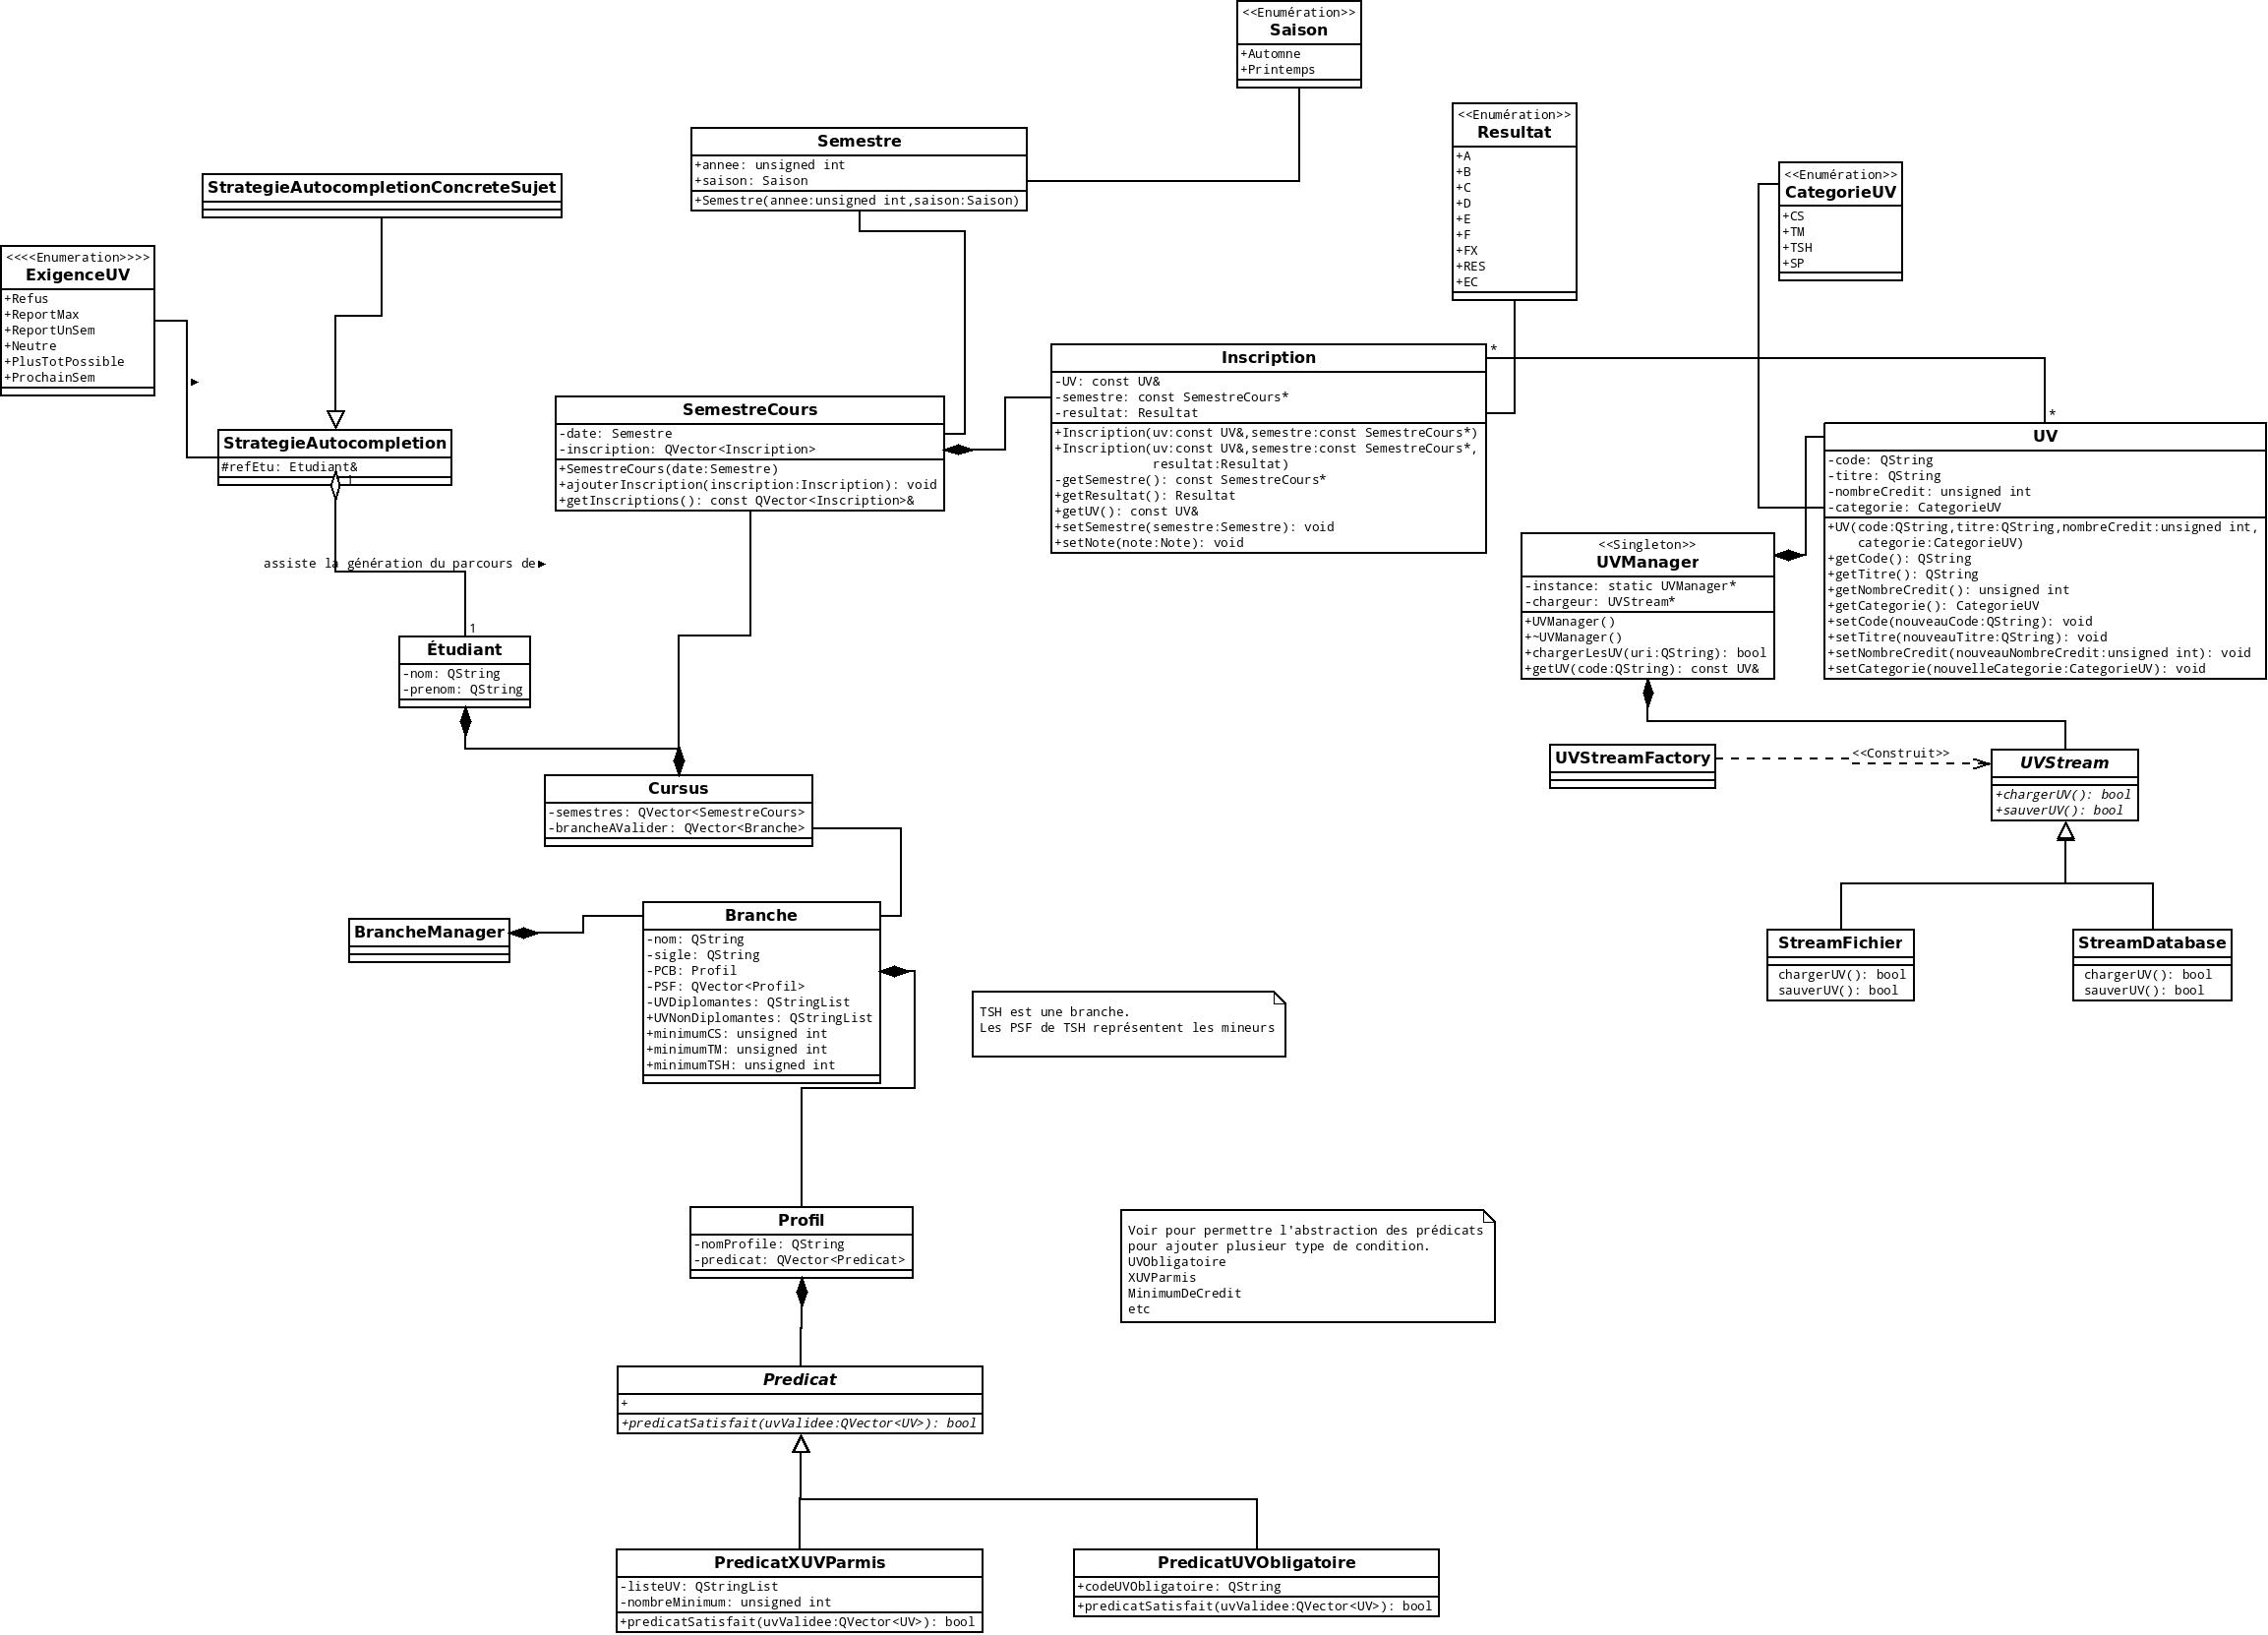
\includegraphics[scale=0.18]{utprofiler}
				\end{center}
			\end{figure}
            
\end{document}
